\documentclass[9pt]{beamer}

\geometry{paperwidth=213.3mm,paperheight=120mm}

\usetheme[{titleformat plain}=smallcaps,
           titleformat title=smallcaps,
           titleformat subtitle=regular,
           titleformat section=smallcaps,
           titleformat frame=smallcaps,
           % numbering=fraction,
          ]{metropolis}
% \usepackage{appendixnumberbeamer}

\definecolor{mLightGreen}{HTML}{14B03D}
\definecolor{vpGreen}{HTML}{66c2a5}
\definecolor{vpOrange}{HTML}{fc8d62}
\providecommand{\iRef}[1]{{\color{mLightGreen}\small $[$#1$]$}}

\usepackage{booktabs}
\usepackage[scale=2]{ccicons}

\usepackage{../_style/common}
\usepackage{../_style/defs}

\usepackage{tikz}
\usetikzlibrary{shapes,arrows}
\usepackage{amsmath, bm}
\usepackage{siunitx}
\usepackage{physics,hepnames}
\usepackage{mathtools}
\usepackage{enumitem}
\setenumerate[1]{%
      label=\protect\usebeamerfont{enumerate item}%
      \protect\usebeamercolor[fg]{enumerate item}%
      \insertenumlabel.}
\setitemize{label=\usebeamerfont*{itemize item}%
    \usebeamercolor[fg]{itemize item}
      \usebeamertemplate{itemize item}}

\usepackage{subfig}
\usepackage{colortbl}
\usepackage{multirow}
\usepackage{pifont}

\usepackage{pgfplots}
\usepgfplotslibrary{dateplot}

\usepackage{ulem}

\graphicspath{{pictures/}}

\title{PDF sampling}
\subtitle{as \sout{Bayesian} na\"ive as possible}
\date{August, 2022}
\author{\textit{\textbf{Alessandro Candido}}, Luigi Del Debbio, Tommaso Giani, Giacomo Petrillo}
%\institute{N3PDF}
\titlegraphic{
    \raisebox{10pt}[0pt][0pt]{
\includegraphics[width=2.5cm]{../_logos/nnpdf_logo.pdf}}\hspace*{10pt}
    \hfill
    \raisebox{5pt}[0pt][0pt]{
\includegraphics[height=0.8cm]{../_logos/n3pdf_logo.pdf}}\hspace*{10pt}
    
\includegraphics[height=1.3cm]{../_logos/erc_logo1.png}

    \vfill\vspace*{230pt}
    
\includegraphics[height=1cm]{../_logos/unimi_logo.png}\hfill
    
\includegraphics[height=1cm]{../_logos/infn_logo.png}\\
    \vspace*{5pt}
    {
        \fontsize{3pt}{3.5pt}\selectfont
        \begin{center}
            This project has received funding from the European Union's Horizon
            2020 research and innovation programme under grant agreement No
            740006\quad 
\includegraphics[height=5pt]{../_logos/eu-flag.jpg}
        \end{center}
    }
}

\begin{document}

\maketitle

\setlist[description]{font=\quad\normalfont\bfseries\scshape\space}
\metroset{block=fill}

\begin{frame}{Function space}
    \begin{columns}
        \begin{column}{0.5\textwidth}
            A function $f: \mathbb{R} \to \mathbb{R}$ (or suitable intervals)
            lives in an infinite-dimensional space.
            \vspace*{20pt}

            This has a simple consequence:
            \begin{block}{Under-determination}
                Fitting an \textbf{unknown function} on a finite number of data
                is always an \textbf{under-determined} problem.
            \end{block}
            \vspace*{20pt}

            How to choose a solution, when \alert{many} are available and
            \alert{equivalent}?
        \end{column}
        \begin{column}{0.5\textwidth}
            \begin{figure}
                \centering
                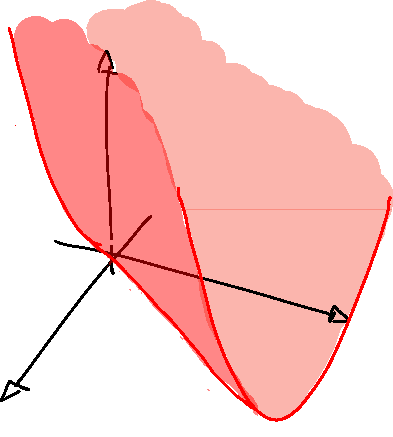
\includegraphics[width=0.6\textwidth]{underdetermined}
                \caption{Possible $\chi^2$ profile in 2D parameter space.}
            \end{figure}
        \end{column}
    \end{columns}
\end{frame}

\begin{frame}{Solutions in the Assumptions}
    \vspace*{10pt}
    \begin{center}
        There are two main ways to attack the problem.
    \end{center}
    \vspace*{10pt}

    \begin{columns}
        \begin{column}{0.5\textwidth}
            1. One consists in \textit{reducing the number of parameters}, by
            \textbf{slicing} a suitable \textbf{hyperplane}.
            \footnote{Not containing zero-directions.}
            \vspace*{10pt}

            This is what we do in PDFs when choosing a \alert{\textbf{fixed
            parametrization}}: we decide which parameters to fit, and take a
            single given value for everything else.
            \vspace*{10pt}

            \begin{figure}
                \centering
                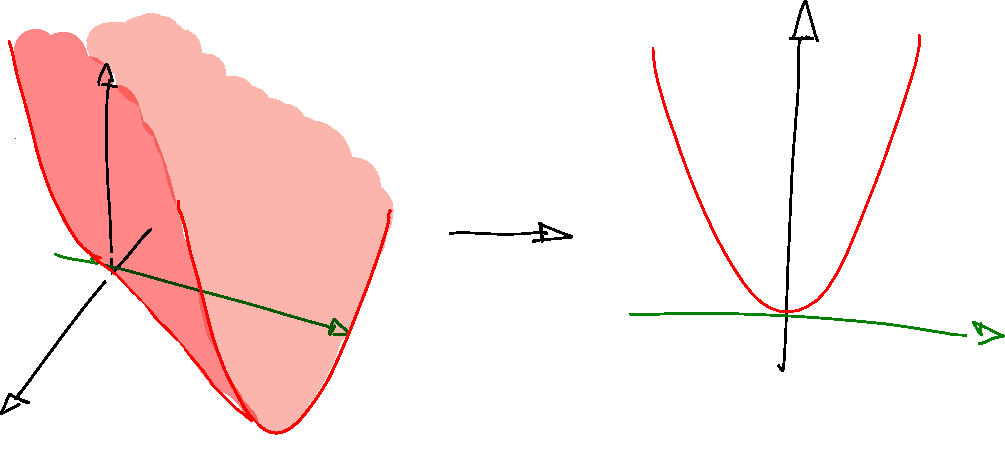
\includegraphics[width=0.8\textwidth]{sliced}
                \caption{$\chi^2$ profile in sliced parameter space.}
            \end{figure}
            \vspace*{10pt}
        \end{column}
        \begin{column}{0.5\textwidth}
            2. The second approach removes the zero-direction by adding
            \textbf{regularization}.
            \vspace*{10pt}

            This is what the \alert{\textbf{Neural Network}} (and its training
            algorithm) is doing under the hood.
            \vspace*{10pt}

            \begin{figure}
                \centering
                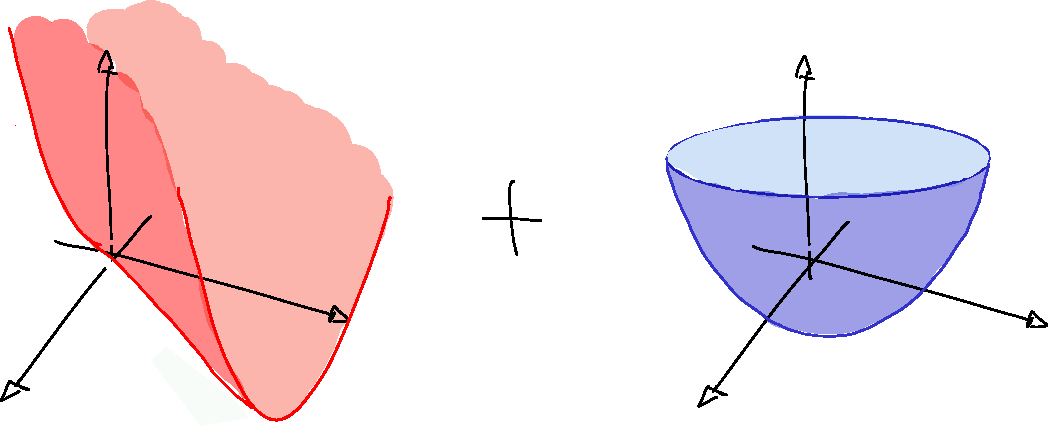
\includegraphics[width=0.8\textwidth]{regularized}
                \caption{$\chi^2$ profile plus regularization function.}
            \end{figure}
        \end{column}
    \end{columns}
\end{frame}

\begin{frame}{So Which?}
    \vspace*{30pt}
    \begin{columns}
        \begin{column}{0.5\textwidth}
            Then which one should we choose?
            \vspace*{10pt}

            \begin{figure}
                \centering
                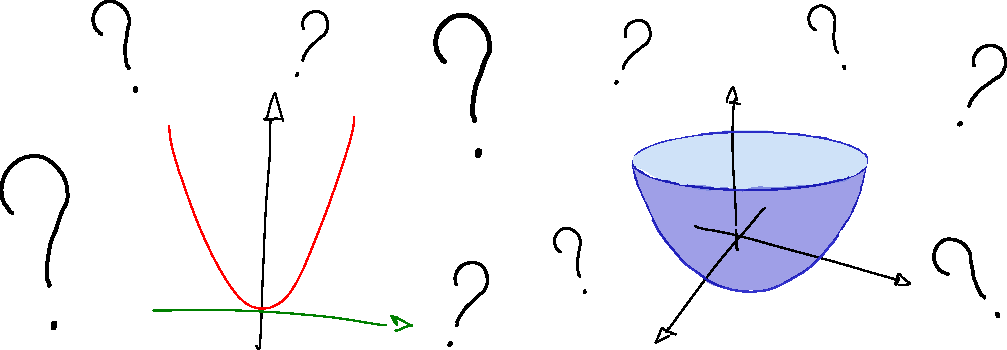
\includegraphics[width=0.8\textwidth]{choice}
            \end{figure}

            \vspace*{10pt}
            There is \textbf{not} an \alert{\textbf{absolute best answer}},
            because both procedures might be \textit{\textbf{arbitrary}}.
        \end{column}
        \begin{column}{0.5\textwidth}
            So, we need a guiding principle to make a good choice, and a good one is:
            \begin{center}
                \itshape
                \bfseries
                Choices should encode physics assumptions
            \end{center}
            and as little arbitrariness as possible\footnote{
                Though nothing is actually bias-free, so better to know and
                declare your bias, rather than hiding it.
            }.

            \vspace*{20pt}
            So what about PDFs?
            \begin{description}
                \item[cuts] cutting the space (fixed parametrization) is no
                    bad, \textbf{if you know how to do it}: you need
                    \alert{\textbf{precise theoretical insight}} on the
                    \alert{\textbf{\pdf shape}}
                \item[regularization] also this need as much motivation as the
                    former, but it makes \textit{to shift the focus} from the
                    exact shape to more abstract \alert{\textbf{features}}
            \end{description}
            \vspace*{20pt}
        \end{column}
    \end{columns}
\end{frame}

\begin{frame}{The NN}
    \begin{center}
        What is then doing the neural network (NN)? Why is it working so well?
    \end{center}
    \vspace*{10pt}

    \begin{columns}
        \begin{column}{0.5\textwidth}
            \begin{figure}
                \centering
                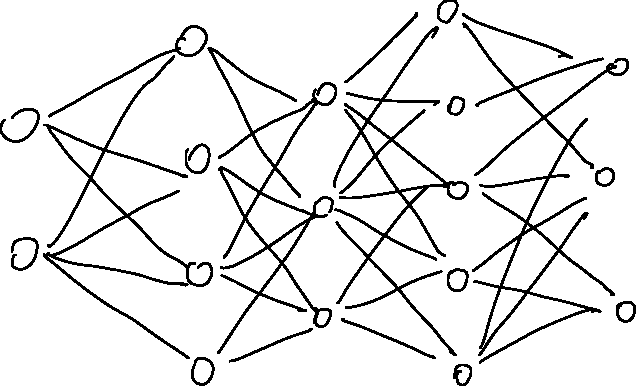
\includegraphics[width=0.6\textwidth]{nn}
            \end{figure}
            "working" is a bit ambiguous, but tests are helpful to develop
            enough trust.

            \vspace*{10pt}
                Essentially, the \textit{NN is encoding} an
                \alert{\textbf{interpolation hypothesis}} \textit{in the
                architecture \textbf{and} training algorithm}.
        \end{column}
        \begin{column}{0.5\textwidth}
            While both the approaches are limiting \textit{model complexity},
            the \textbf{Neural Network} is able to \textbf{follow data trends}.

            \vspace*{10pt}
            \begin{exampleblock}{Physical Wiggles}
                A criticism we collected has been about \textit{NN opaque
                assumptions} might \textbf{prevent} to follow \textbf{small
                physical fluctuations}, but it is actually the other way
                round:\footnote{In principle, yet to be proven in practice.}

                \begin{description}
                    \item[fixed param.] in this case, you can only find
                        oscillations you are allowing for, so you need to know
                        in advance \textbf{each and every wiggle} to
                        discriminate physical ones from noise
                    \item[NN] all wiggles are deweighted, but physical wiggles
                        should be resolved more and more by data, so
                        \textit{"enough precision"} in the
                        \alert{\textbf{data}} will naturally
                        \textbf{\alert{overwhelm} the theoretical
                        \alert{(learning) bias}}
                \end{description}
            \end{exampleblock}
        \end{column}
    \end{columns}
\end{frame}

\begin{frame}{Looking for Insights}
    \begin{columns}
        \begin{column}{0.5\textwidth}
            \textit{NNPDF "framework"} is much \textbf{\textit{more}} than a Neural
            Network only:
            \begin{itemize}
                \item nice representation of a generic distribution (\textbf{replicas})
                \item many \textbf{tests} in place
                \item \textbf{fast theory} framework
                \item \textbf{lots of data} implemented
                \begin{itemize}
                    \item both theory calculation and
                    \item commondata implementation with uncertainties
                        (including correlated systematics)
                \end{itemize}
                \item and more\dots
            \end{itemize}
            \vspace*{10pt}

            \begin{center}
                \itshape
                We do \textbf{not} want to \textbf{loose} \alert{\textbf{any}} of these.
            \end{center}
        \end{column}

        \begin{column}{0.5\textwidth}
            But sometimes we \textbf{lack insight}: we have tests for this, but
            they are not always a handy tool to answer all questions.
            \vspace*{10pt}

            \begin{exampleblock}{Hopscotch}
                \begin{center}
                    \itshape
                    What are our criticism to CT replicas?
                \end{center}
                Mostly we blame the method, but little criticism on the result.

                Some \textbf{physical assumptions} have been checked:
                \begin{itemize}
                    \item $\chi^2$ vs $\chi^2_{t_0}$
                    \item integrability and sum rules
                    \item positivity
                \end{itemize}

                But it might be hidden in the NN \textbf{regularization}.
            \end{exampleblock}

        \end{column}
    \end{columns}

    \vspace*{10pt}
    Another limitation\footnote{
        Actually, this is where everything started from.
    } is that the current methodology need to make a \textbf{fit to \alert{one
    sample} at a time}. The distribution is only the result of many fits.
    \textit{\textbf{What if we could fit the distribution all at once?}}
    \vspace*{-10pt}
\end{frame}

\begin{frame}{Restart from Bayes}
    Typical examples of ML are image and speech recognition, generative tasks,
    style transfer and so on.

    All these problems have in common very high dimensional objects, with poor
    analytical insight on its structure. Working out an explicit and effective
    representation for them is difficult.

    This is not the case of PDF: we already describe them with a math language,
    and we have clear analytic properties at hand (sum rules, power-like
    behavior, and so on).
    
    ---

    Then, (Bayes).

    \begin{equation*}
        P(A|B) = \frac{P(B|A) P(A)}{P(B)}
    \end{equation*}
    
    Advantage: an explicit prior will do what the NN is now doing.
\end{frame}

\begin{frame}{Prior Choice \& Implementation}
    Gaussian process
    
    ---

    Fit Basic idea: take a bunch of points out of the function, the rest comes
    by interpolation. Which ones? LHAPDF's of course :)
\end{frame}


\begin{frame}{(Very) Preliminary Results}
    \vspace*{10pt}
    \begin{figure}
        \centering
        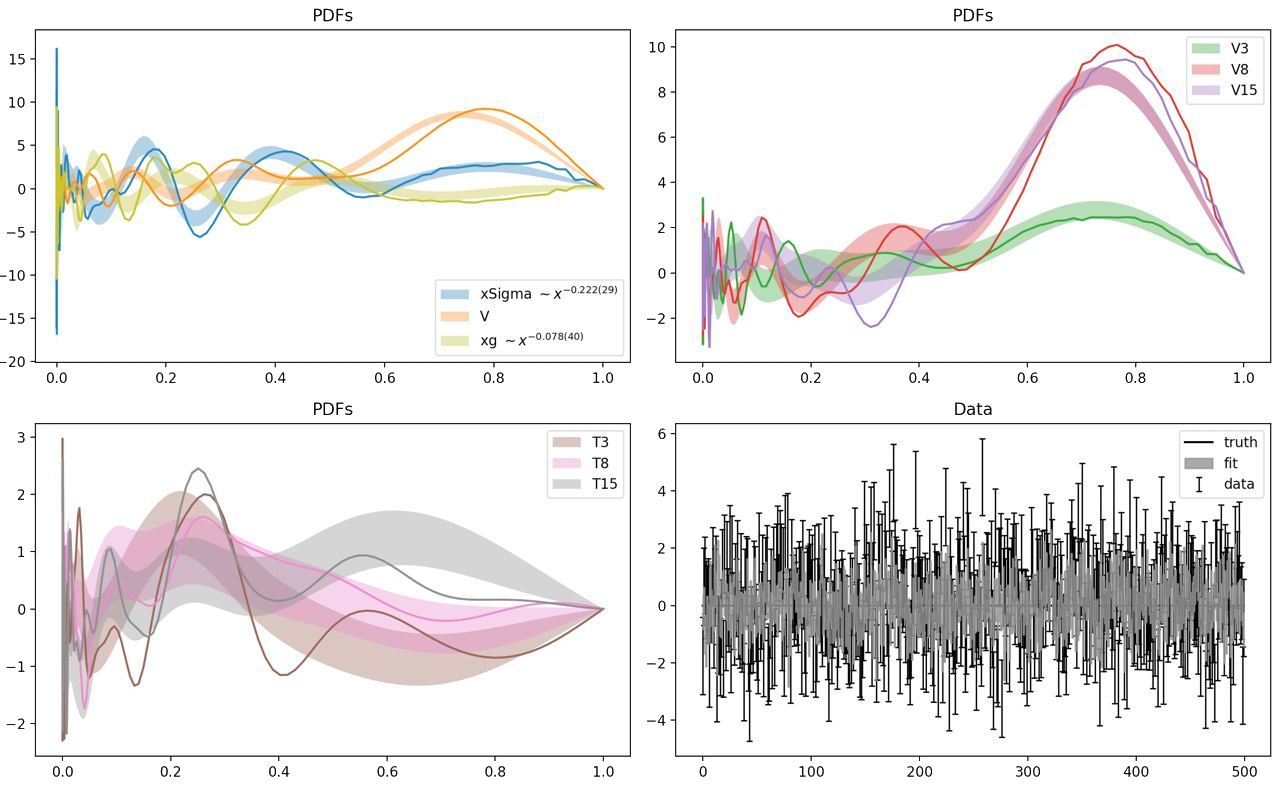
\includegraphics[width=0.75\textwidth]{fit-pdf}
        \caption{
            Even with completely random data and theory, we get a valence like
            structure (\textbf{valence peak}, wrong place, wrong height) by
            virtue of \textbf{sum rules}. Still, they are too much
            unconstrained to get correct values.
        }
    \end{figure}
\end{frame}

\begin{frame}[standout]
    Questions?
\end{frame}

\appendix

\begin{frame}{PDF features}
    \begin{description}
        \item[sum rules] analytically, zero errors data point on the primitive
        \item[quadratic points] least square fit
        \item[PDF positivity] we can fit the log processes
    \end{description}
\end{frame}

\begin{frame}{Further results}
    \vspace*{30pt}
    \begin{columns}
        \begin{column}{0.6\textwidth}
            \begin{figure}
                \centering
                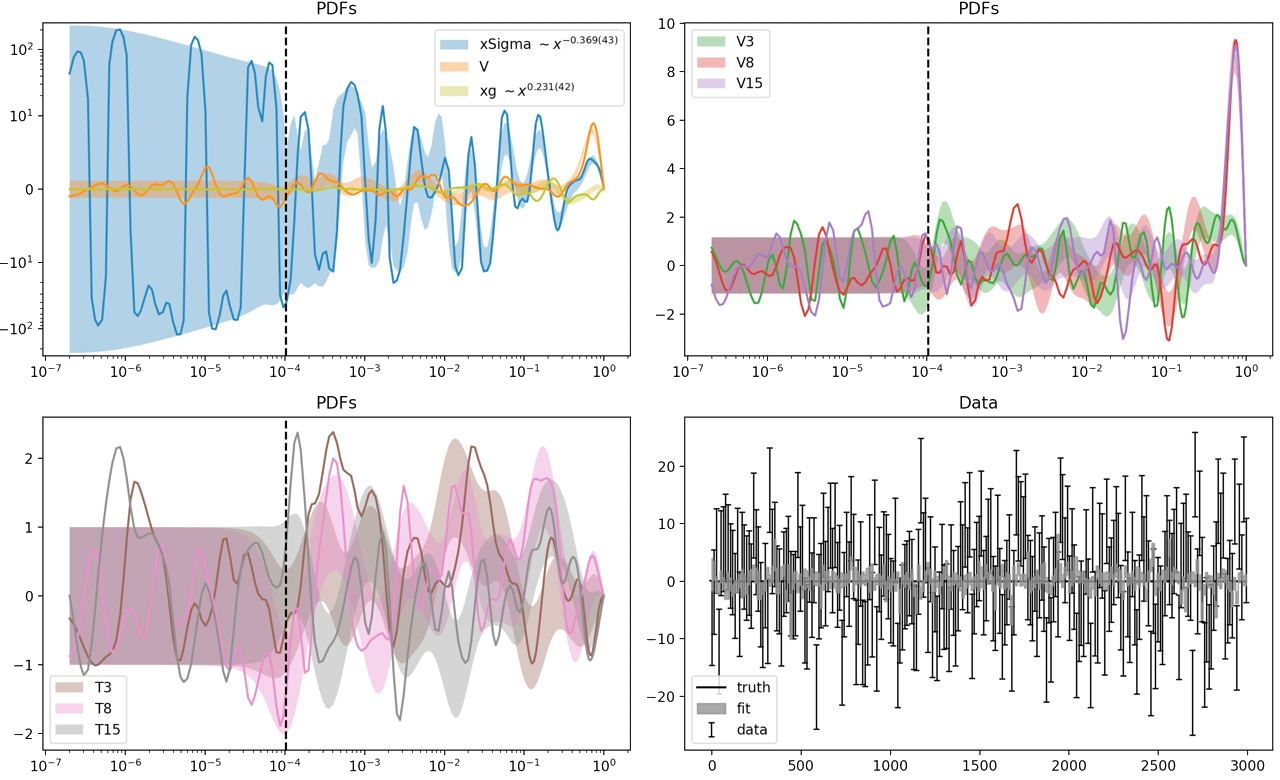
\includegraphics[width=\textwidth]{fit-pdf-new}
                \caption{
                    New fit candidate, with less random data (still pretty
                    random).
                }
            \end{figure} 
        \end{column}
        \begin{column}{0.4\textwidth}
            \begin{figure}
                \centering
                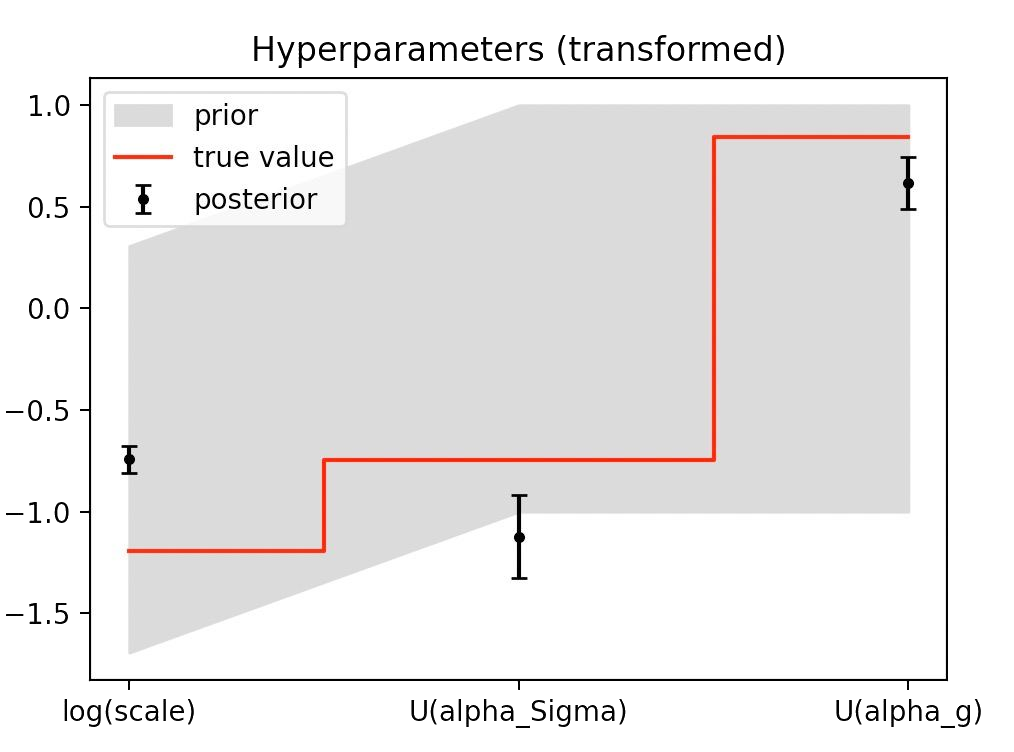
\includegraphics[width=\textwidth]{fit-hyper-new}
                \caption{
                    Hyperparameters fit: notice that while exponents are
                    working, we are still missing the correlation length.
                }
            \end{figure} 
        \end{column}
    \end{columns}
\end{frame}

\begin{frame}{Tests}
    First: , because we don't know the answer. Closure
    tests are a clue, but we want something to perform well on the truth, and
    not knowing it we are extrapolating from something that is working well on
    a truth candidate.
\end{frame}

\end{document}
